\documentclass{article}
%\usepackage[utf8]{inputenc}
\usepackage{graphicx, amsmath,amssymb,latexsym, booktabs,array,multirow, pgfplots,pgfkeys}
\usepackage{listings}
\usepackage{hyperref}
\hypersetup{
    colorlinks=true,
    linkcolor=blue,      
}
\usepackage{tikz}
\usepackage{cite}
\usepackage
[
        a4paper,% other options: a3paper, a5paper, etc
        left=2.5cm,
        right=2.5cm,
        top=2cm,
        bottom=2cm,
        % use vmargin=2cm to make vertical margins equal to 2cm.
        % us  hmargin=3cm to make horizontal margins equal to 3cm.
        % use margin=3cm to make all margins  equal to 3cm.
]{geometry}
\DeclareMathOperator*{\argmax}{argmax}
\title{neural networks}
\author{tanvisahay31 }
\date{November 2015}

\usepackage{natbib}
\usepackage{graphicx}
\usepackage{tikz}
\begin{document}

%\hrule height 1pt
\vspace{0.5em}
\begin{center}
%\large{CS585 : Introduction to Natural Language Processing}\\
%\vspace{1.4em}
\large{Data Visualization and Exploration - Homework 2 and 3}\\
\vspace{0.6em}
\large{Submitted By: Tanvi Sahay}
\end{center}
\vspace{0.5em}
%\hrule height 1pt
\noindent
\section*{Visualizations for Facebook Dataset}
The facebook dataset has been visualized using four different types of visualizations: heatmap, histogram, line chart and scatter plot. Options for changing the x-axis of heatmap, data displayed for histogram and y-axis for scatter plot and line chart have been provided as radio buttons. The heat chart shows values of 8 different features with respect to either the type of post, category of post of payment status. Histogram shows the count or frequency of posts, distributed either per month, per weekday, per hour, per category or per type. Scatter plots and line charts show the distribution of Total Comments, Likes or Overall Interactions distributed over post weekdays and post hours respectively. A screenshot of all four visualizations has been shown in figure 1. 

\begin{figure}[h]
\centering
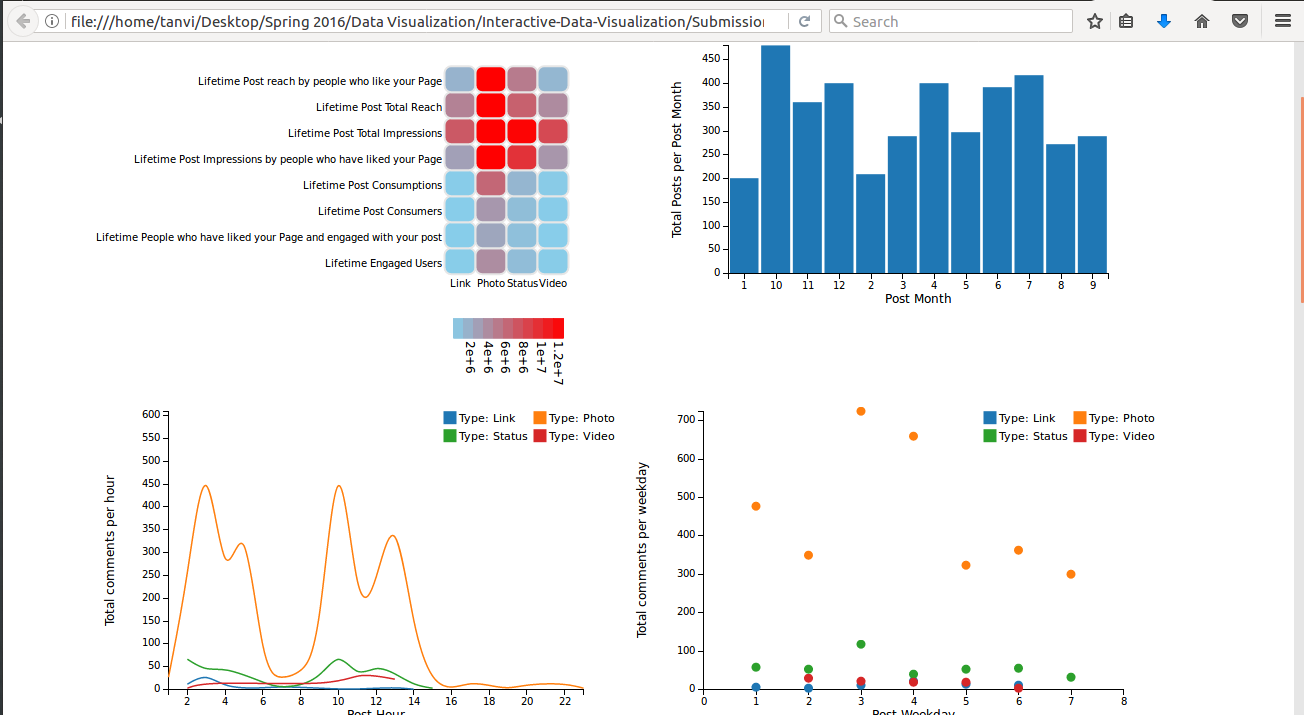
\includegraphics[scale=0.3]{fb_all.png}
\caption{Visualizations for Facebook dataset}
\end{figure} 

\noindent
Each visualization has been provided with both x and y axis, axis labels, ticks, titles and color legends where necessary. All four visualizations can interact with each other, with changes in heatmaps and histograms being reflected in all four plots, along with changes in radio options. Selection works in heatmaps and histograms by clicking on the title of a column or row and in line charts and scatter plots by hovering over the legend object of the category to be displayed. Probing works in all four plots by hovering over the point whose values are to be seen. The library used for these visualizations was dc.js. Explanations for all default visualizations have been provided on the web page itself. 

\subsection*{Data Cleaning and Manipulation}
The facebook dataset had several missing values for the columns "Paid", "like" and "share". These cases of missing values were handled by manually inputting the value '0'. This value was chosen to avoid changes in any statistical computations. Inputting a non-zero value would have caused the statistical compuatations such as sum and count to change, which may have mislead the viewer. For preparing the heatmap, all features and their values were collapsed into two columns, instead of the originally present 8, as it provided better analysis of the features. The columns were collapsed into: (feature, value) with example tuples as: (Lifetime Post Consumption, 553385), (Lifetime Post Consumers, 294124) and so on. Clean up was performed usig python and the updated file was saved as "heatmap\_type\_3.csv". 

\newpage 
\section*{Visualizations for Wine Dataset}
The wine dataset has been visualized using three visualizations: a pie chart showing the number of white and red wines, a bar chart, showing the distribution of total number of wines by quality and a scatter plot showing total alcohol content over the quality distribution for both types of wines. Drop down menus for selecting the x and y axis for the scatter plots have been provided as well. All the plots include labels, axis, tick marks and legends where required. Selection and and probing has also been included and all thee plots can interact with each other, with changes in the pie chart and/or histogram being reflected in all three plots. In depth analysis of this dataset was not performed. However, a cursory glance at the plots provides some interesting information, such as: the number of white wines in the dataset is much more than that of red wines (may be because there are more varieties of white wine in general?). It can also be seen that a majority of wines have the quality 6. Also, from the scatter plot, it can be seen that white wines in general have a much higher alcohol content than red wines, especially in the range of quality 5-7, which is where most wines lie. A derived hypothesis from these two observations can be that majority of white wines(which lie in the quality 5-7 range) have a high alcohol content as opposed to red wines, which in general have a low alcohol content. More such trends can be seen by changing the x and y axis. 

\subsection*{Data Manipulation}
Since the dataset had no missing values, no cleaning was required. However, for easier access of data, both the red and white wine datasets were merged into one. An additional column 'type' was created and the type of wine i.e. red or white was filled into it, along with the data from both csv files for individual wine types. This manipulation was done using Python and the final file was saved as "wine\_all.csv". A screenshot of the plots generated for this data has been included as figure 2.

\begin{figure}[h]
\centering
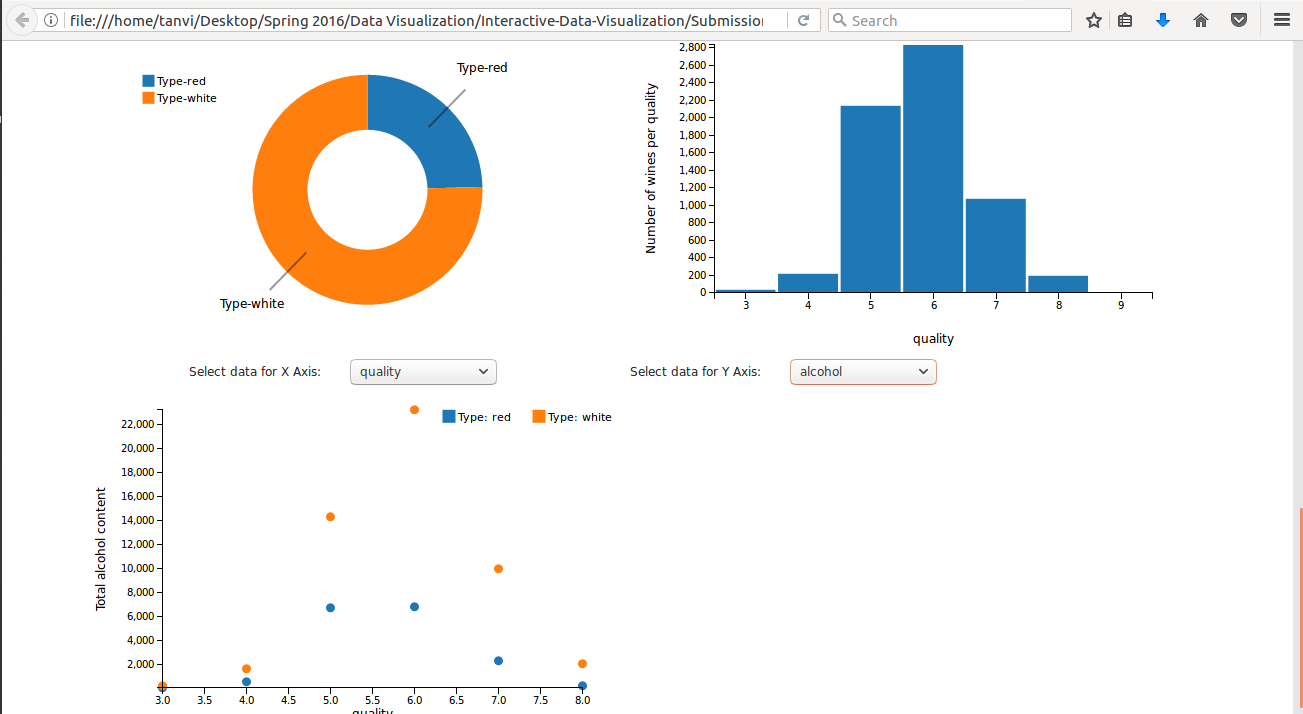
\includegraphics[scale=0.3]{wine_all.png}
\caption{Visualizations for Wine Dataset}
\end{figure}

\section*{Additional Visualizations for Facebook Dataset}

Three additional visualizations have also been provided along with the ones already shown earlier. No analysis was done on these. Labels, Axis, ticks and probing is present in all three. The first visualizatin is a line chart with two y axis, one on the left and one on the right. It shows Lifetime Post Reach vs Lifetime Post Impressions per Month and can be accessed by the button ``visualization 1". The second visualization is a scatter plot showing the number of people to like a post for each post, categorized by weekday. This can be accessed by the button ``visualization 2". The last one is a pie chart showing the count of each type of data i.e. Photo, Status, Link and Video. Each pie slice can be clicked to highligh it and show its label. The labels of the two highest types are visible by default. This final visualization can be accessed by the button ``visualization 3". 
\end{document}

